\documentclass[12pt,aspectratio=43,dvipsnames,table]{beamer}
\usepackage[T1]{fontenc}
\usepackage[utf8]{inputenc}
\usepackage[francais]{babel}
\usepackage{url}
\usepackage{multirow}
\usepackage{mathtools}
\usepackage{CJKutf8}
\usepackage{arabtex}
\usepackage{appendixnumberbeamer}


\usetheme{default}
\useinnertheme{default}
\useoutertheme{default}
\usefonttheme{serif}

\usecolortheme[named=RoyalPurple]{structure}

% Marges autour des slides
\setbeamersize{text margin left=5mm, text margin right=5mm}

% Suppression des symboles de navigation
\beamertemplatenavigationsymbolsempty

% Définition du pied de page
\setbeamertemplate{footline} {
  \hfill{
    \insertshortdate ~- %
    page \insertframenumber~sur~\inserttotalframenumber %
    %\hspace*{0.1cm}
  } \vspace*{0.05cm}
}

% Définition des espacements des listes
\setlength{\leftmargini}{0.6cm}
\setlength{\leftmarginii}{0.4cm}
\setlength{\leftmarginiii}{0.4cm}
\setbeamercolor{itemize subitem}{fg=RubineRed}
\linespread{1.15}

\title{Recherche d'information cross-lingue}
\subtitle{Applications multilingues - module X9IT100}
\author{Florian Boudin}
\institute{Département informatique, Université de Nantes}
\date[14 novembre 2013 / Rév.~2]{Révision~2 du 14 novembre 2013}

% Pour ajouter le plan au début de chaque section
\AtBeginSection[]
{
\begin{frame}
\frametitle{Plan}
\addtocontents{toc}{\protect\vspace*{-0.5em}}
\tableofcontents[sectionstyle=show/shaded,subsectionstyle=hide,subsubsectionstyle=hide]
\end{frame}
}

\begin{document}


%-B--------------------------------------------------------------------------B-%
\frame[plain]{\titlepage}
%-E--------------------------------------------------------------------------E-%


%-B--------------------------------------------------------------------------B-%
\begin{frame}
    \frametitle{Préface}
    \begin{itemize} \itemsep10pt
        \item Volume horaire
        \begin{itemize}
            \item 1 CM - 3 TD/TP
        \end{itemize}
        \item Notions abordées dans ce cours~:
        \begin{itemize}
            \item Rappels des notions de RI.
            \item Sensibilisation aux difficultés liées aux langues.
            \item Présentation de la problématique et des méthodes de RI 
                  cross-lingue.
        \end{itemize}
        \item Ce cours est basé sur le livre \textit{Cross-Language Information 
              Retrieval} de Jian-Yun Nie~\cite{DBLP:series/synthesis/2010Nie}.
    \end{itemize}
\end{frame}
%-E--------------------------------------------------------------------------E-%


%-B--------------------------------------------------------------------------B-%
\begin{frame}
    \frametitle{Introduction}
    \begin{itemize} \itemsep10pt
        \item La \textbf{Recherche d'Information} (RI) fait partie intégrante de
              notre vie quotidienne.
        \item Dans la plupart des cas, nous recherchons des documents rédigés 
              dans notre langue maternelle, en général celle utilisée dans la 
              requête.
        \item \textbf{Cependant...}
        \begin{itemize}
            \item L'information pertinente n'est pas toujours disponible dans 
                  notre langue maternelle.
            \item Le web offre une mine d'information riche et multilingue à 
                  laquelle nous souhaitons avoir accès.
        \end{itemize}
        \item \'Emergence de la problématique de la RI cross-lingue.
    \end{itemize}
\end{frame}
%-E--------------------------------------------------------------------------E-%


%##############################################################################%
\section{Rappels des notions de RI}
%##############################################################################%


%-B--------------------------------------------------------------------------B-%
\begin{frame}
    \frametitle{Le processus de recherche d'information}
    \begin{figure}
    \centering
    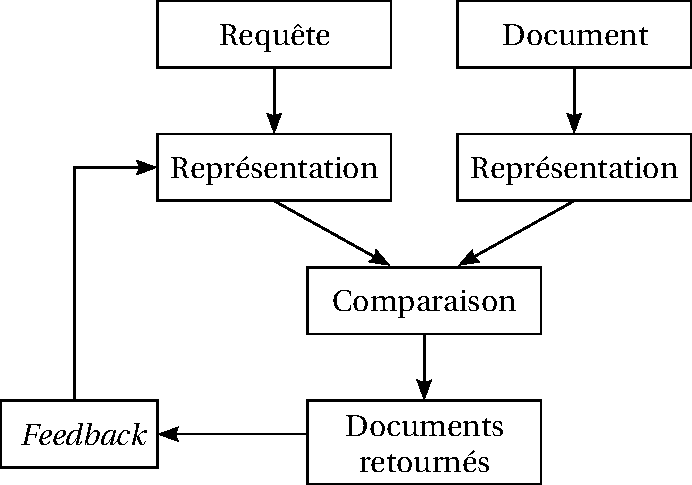
\includegraphics[width=0.75\textwidth]{img/typicalIR.pdf}
    \caption{Processus de recherche d'information (Figure 1.1 
             de~\cite{DBLP:series/synthesis/2010Nie}).}
    \end{figure}
\end{frame}
%-E--------------------------------------------------------------------------E-%


%-B--------------------------------------------------------------------------B-%
\begin{frame}[allowframebreaks]
    \frametitle{Modèles de RI}
    \begin{itemize} \itemsep10pt
        \item Un modèle définit la représentation des documents et des requêtes 
              ainsi que la fonction de pondération.
        \item La plupart des modèles sont construits sur la notion de 
              \textit{terme}, qui peut être un mot (e.g.~\textit{computer}), un 
              stem (e.g.~\textit{comput}) ou une expression multimots 
              (e.g.~\textit{computer system}).

        \framebreak

        \item \textbf{Modèle booléen}
        \begin{itemize}
            \item Les documents sont représentés par une conjonction de termes, 
                  e.g.~$D = t_1 \land t_2 \land t_3$ qui signifie que les termes
                  $t_1$, $t_2$ et $t_3$ apparaissent dans $D$.
            \item Une requête est représentée par une expression booléenne, 
                  e.g.~$Q = (t_1 \land t_2) \lor t_3$.
            \item Un document est considéré comme pertinent si et seulement si 
                  il y a l'implication logique $D \Rightarrow P$.
        \end{itemize}

        \framebreak

        \item \textbf{Modèle vectoriel}~\cite{DBLP:journals/cacm/SaltonWY75,DBLP:books/mg/SaltonG83}
        \begin{itemize}
            \item Les documents et requêtes sont représentés par des vecteurs 
                  dans un espace vectoriel composé de tous les termes.
            \item Dans chaque vecteur, chaque élément ($d_i$ ou $q_i$, 
                  $1 \leq i \leq n$) représente le poids du terme.
        \end{itemize}
        %
        \vspace*{-0.5em}
        \begin{align*}
          \text{espace vectoriel~:} &~(t_1, t_2, \cdots, t_n) \\
          \text{document~:} &~(d_1, d_2, \cdots, d_n) \\
          \text{requête~:} &~(q_1, q_2, \cdots, q_n)
        \end{align*}
        \vspace*{-1.5em}
        %
        \begin{itemize}
            \item Les poids des termes peuvent être binaires, i.e.~1 pour la 
                  présence et 0 l'absence, ou calculés avec $tf \times idf$.

            \framebreak

            \item La pertinence des documents est habituellement calculée avec 
                  une mesure de similarité cosinus.
        \end{itemize}
        %
        \begin{align*}
          \text{sim}(d,q) = &~\frac{ \mathbf{d} \cdot \mathbf{q} }
                                   { \left\|\mathbf{d}\right\| 
                                     \left\|\mathbf{q}\right\| } \\[0.5em]
                          = &~\frac{ \sum _{i=1}^n d_i q_i }
                                   { \sqrt{\sum_{i=1}^n d_i^2}
                                     \sqrt{\sum _{i=1}^n q_i^2} }
        \end{align*}

        \framebreak

        \item \textbf{Modèle probabiliste}~\cite{robertson1976relevance}
         \begin{itemize}
            \item Le score de pertinence d'un document $D$ par rapport à une 
                  requête $Q$ est estimé à partir de $P(\text{pertinence}|D,Q)$,
                  la probabilité de pertinence de $D$ par rapport à $Q$.
            \item Okapi BM25~\cite{DBLP:conf/trec/RobertsonWHGL92} est le modèle 
                  le plus utilisé.
            \begin{equation*}
              \text{score}(D,Q) = \sum_{i=1}^{n} \text{idf}(q_i) \cdot 
              \frac{f(q_i, D) \cdot (k_1 + 1)}
              {f(q_i, D) + k_1 \cdot (1 - b + b \cdot \frac{|D|}{\text{avgdl}})}
            \end{equation*}
            \item où $f(q_i, D)$ est la fréquence du terme $q_i$ dans $D$, 
                  $avgdl$ est la longueur moyenne des documents, 
                  $k_1 \in [1.2,2.0]$ et $b = 0.75$.
        \end{itemize}

        \framebreak

        \item \textbf{Modèle de langue}~\cite{DBLP:conf/sigir/PonteC98}
        \begin{itemize}
            \item Utiliser $P(D|Q)$ pour estimer le score de pertinence d'un 
                  document $D$ par rapport à une requête $Q$.
            \item Avec le théorème de Bayes, nous avons~:
            \begin{equation*}
              P(D|Q) = \frac{P(Q|D)P(D)}{P(Q)} \propto P(Q|D)P(D)
            \end{equation*}
            \item En considérant les termes de la requêtes comme indépendants~:
            \begin{equation*}
              P(Q|D) = \prod_{t_i \in Q} P(t_i | D)
            \end{equation*}
            \item $P(t_i | D)$ est estimée par un modèle de langue du document.
        \end{itemize}

    \end{itemize}
\end{frame}
%-E--------------------------------------------------------------------------E-%


%-B--------------------------------------------------------------------------B-%
\begin{frame}
    \frametitle{\'Evaluation}

    \begin{align*}
    \text{precision} & = \frac{\text{\# documents pertinents retrouvés}}
                              {\text{\# documents retrouvés}}
                              \\[1.5em]
    \text{rappel} & = \frac{\text{\# documents pertinents retrouvés}}
                           {\text{\# documents pertinents dans la collection}}
                           \\[1.5em]
    \text{MAP} & = \overbracket[1pt]{
                      \frac{1}{M} \sum_{j=1}^{M}
                   }^{\forall~\text{requêtes}} 
                   \underbracket[1pt]{
                    \Bigg( \frac{1}{N_j} \sum_{i=1}^{N_j} pr(d_{ij}) \Bigg)
                   }_{
                      \substack{
                        \text{moyenne des précisions} \\ 
                        \text{aux rangs des documents} \\ 
                        \text{pertinents}
                      }
                    }
    \end{align*}

\end{frame}
%-E--------------------------------------------------------------------------E-%


%##############################################################################%
\section{Les difficultés liées aux langues}
%##############################################################################%


%-B--------------------------------------------------------------------------B-%
\begin{frame}
    \frametitle{Introduction}
    \begin{itemize} \itemsep10pt
      \item Les travaux en RI ont longtemps porté uniquement sur les langues 
            européennes.
      \item Cette situation a changée avec l'avènement du web et la 
            disponibilité de grandes collections de documents dans de nombreuses 
            langues.
      \item Les traitements ``basiques'' développés pour les langues 
            européennes sont en partie ré-utilisables pour d'autres langues, 
            mais certaines nécessitent des traitements spécifiques.
    \end{itemize}
\end{frame}
%-E--------------------------------------------------------------------------E-%


%-B--------------------------------------------------------------------------B-%
\begin{frame}
    \frametitle{Le processus de recherche d'information}
    \begin{figure}
    \centering
    \includegraphics<1>[width=0.75\textwidth]{img/typicalIR.pdf}
    \includegraphics<2>[width=0.769\textwidth]{img/preprocIR.pdf}
    \caption{Processus de recherche d'information (Figure 1.1 
             de~\cite{DBLP:series/synthesis/2010Nie}).}
    \end{figure}
\end{frame}
%-E--------------------------------------------------------------------------E-%


%-B--------------------------------------------------------------------------B-%
\begin{frame}[shrink=5]
    \frametitle{Langues européennes}
    \framesubtitle{Stemming (racinisation)}
    \begin{itemize} \itemsep10pt
        \item Porter~\cite{porter1980algorithm} et Krovetz~\cite{Krovetz:1993}
              pour l'anglais.
        \item Snowball\footnote{\url{http://snowball.tartarus.org/}}~: extension
              de l'algorithme de Porter à 15 langues.
        \begin{itemize}
            \item \textbf{Langues romanes} (fr, es, pt, it, ro) \\
                  \quad e.g.~contradictoires $\to$ contradictoir (fr) \\
            \item \textbf{Langues germaniques} (de, nl) \\
                  \quad e.g.~aufeinanderschlügen $\to$ aufeinanderschlug (de)
            \item \textbf{Langues scandinaves} (se, no, da) \\
                  \quad e.g.~klostergården $\to$ klostergård (se)
            \item \textbf{Autres langues} (ru, fi)\\
                  \quad e.g.~edeltäjälleen $\to$ edeltäj (fi) \\
        \end{itemize}
        \item Permet souvent une meilleure précision mais les moteurs de 
              recherche actuels ne l'utilisent pas.
    \end{itemize}
\end{frame}
%-E--------------------------------------------------------------------------E-%


%-B--------------------------------------------------------------------------B-%
\begin{frame}[shrink=5]
    \frametitle{Langues européennes}
    \framesubtitle{Decompounding (décomposition)}
    \begin{itemize} \itemsep10pt
        \item Dans les langues agglutinantes (e.g.~Allemand, Néerlandais, 
              Finnois), les mots se forment à partir d'une racine lexicale à 
              laquelle on peut ajouter un certain nombre d'affixes.
        \begin{itemize}
            \item[e.g.] \textit{hungerstreiks} (de) est composé de 
                  \textit{hunger} (faim), \textit{strieks} (grève) et peut aussi
                  s'écrire en deux mots séparés.
        \end{itemize}
        \item De multiples expressions d'un même concept peuvent engendrer des 
              \textit{mismatches} entre les documents et la requête.
        \item Le processus de \textit{decompounding} correspond à la détection 
              des mots constituants.
        \begin{itemize}
            \item Difficulté liée à l'ambiguïté des mots, par exemple 
                  \textit{hungerstreiks} contient les mots suivants~: 
                  \textit{erst}, \textit{hung}, \textit{hunger}, 
                  \textit{hungers}, \textit{hungerst}, \textit{reik}, 
                  \textit{reiks}, \textit{streik}, \textit{streiks}
        \end{itemize} 
    \end{itemize}
\end{frame}
%-E--------------------------------------------------------------------------E-%


%-B--------------------------------------------------------------------------B-%
\begin{frame}
    \frametitle{Langues asiatiques}
    \framesubtitle{Découpage en mots}
    \begin{itemize} \itemsep10pt
        \item Le Chinois, Japonais et Coréen (\textit{CJK languages}) partagent 
              un héritage commun du aux liens culturels et linguistiques entre 
              ces pays.
        \item Utilisation d'idéogrammes (cn), de kanjis/kanas (jp) ou de 
              hanjas/hangeul (ko).
        \item Une caractéristique des textes chinois et japonais est l'absence 
              d'espaces pour délimiter les mots.
    \end{itemize}
\end{frame}
%-E--------------------------------------------------------------------------E-%


%-B--------------------------------------------------------------------------B-%
\begin{frame}[shrink=5]
    \frametitle{Langues asiatiques}
    \framesubtitle{L'ambiguïté du découpage en mots}
    \begin{CJK*}{UTF8}{gbsn}
    \begin{table}
      \small
      \setlength{\tabcolsep}{2pt}
      \renewcommand{\arraystretch}{1.2}
      \begin{tabular}{ c|c|c|c|c|c|c|c|c|c|c|c l }
      公路局正在 & 治 & 理 & 解 & 放 & 大 & 道 & 路 & 面 & 积 & 水 & 问题。\\
      ~ & 治 & 理 & ~ & ~ & ~ & ~ & ~ & ~ & ~ & ~ & ~ & Aménager \\
      ~ & ~ & 理 & 解 & ~ & ~ & ~ & ~ & ~ & ~ & ~ & ~ & Comprendre \\
      ~ & ~ & ~ & 解 & 放 & ~ & ~ & ~ & ~ & ~ & ~ & ~ & Libération \\
      ~ & ~ & ~ & ~ & 放 & 大 & ~ & ~ & ~ & ~ & ~ & ~ & \'Elargir \\
      ~ & ~ & ~ & ~ & ~ & 大 & 道 & ~ & ~ & ~ & ~ & ~ & Avenue \\
      ~ & ~ & ~ & ~ & ~ & ~ & 道 & 路 & ~ & ~ & ~ & ~ & Route \\
      ~ & ~ & ~ & ~ & ~ & ~ & ~ & 路 & 面 & ~ & ~ & ~ & Couche de surface \\
      ~ & ~ & ~ & ~ & ~ & ~ & ~ & ~ & 面 & 积 & ~ & ~ & Superficie \\
      ~ & ~ & ~ & ~ & ~ & ~ & ~ & ~ & ~ & 积 & 水 & ~ & Accumulation
      \end{tabular}
      \caption{Exemple illustrant la difficulté~du découpage en mots~\cite{li2006}.}
    \end{table}
    \end{CJK*}
\end{frame}
%-E--------------------------------------------------------------------------E-%


%-B--------------------------------------------------------------------------B-%
\begin{frame}
    \frametitle{Langues asiatiques}
    \framesubtitle{Plusieurs types d'ambiguïtés~\cite{wang:approche:recital13}}
    \begin{itemize} \itemsep10pt
        \item Ambiguïté de segmentation en mots
        \begin{CJK}{UTF8}{min}
        \begin{itemize}
          \item[e.g.] わたしはフランス人です。 (jp)
          \item[$\to$] わたし~/~は~/~フランス人~/~です (watashi wa furansujin desu)
        \end{itemize}
        \end{CJK}
        \begin{CJK}{UTF8}{gbsn}
        \begin{itemize} 
          \item[e.g.] 薄熙来自 (cn)
          \item[$\to$] 薄~/~熙来~/~自 (Bo / Xilai / à~partir de)
          \item[$\to$] 薄~/~熙~/~来自 (Bo / Xi / vient de)
          \item[$\to$] 薄~/~熙~/~来~/~自 (Bo / Xi / vient / depuis)
        \end{itemize}
        \end{CJK}
        \item Ambiguïté de catégorisation
        \begin{CJK}{UTF8}{gbsn}
        \begin{itemize} 
          \item[e.g.] 白雪 (cn)
          \item[$\to$] 白雪 (neige blanche, nom)
          \item[$\to$] 白雪 (Bai Xue, nom propre de personne)
        \end{itemize}
        \end{CJK}
    \end{itemize}
\end{frame}
%-E--------------------------------------------------------------------------E-%


%-B--------------------------------------------------------------------------B-%
\begin{frame}
    \frametitle{Autres langues}
    \begin{itemize} \itemsep10pt
        \item Problématiques de la langue Arabe
        \begin{itemize}
            \item Lettre qui change de forme en fonction de sa position.
            \begin{columns}[c] % the "c" option specifies center vertical alignment
            \column{.35\textwidth}
            \item[e.g.] Forme isolée \RL{`} (ayin) \vspace*{-0.5em}
            \item[$\to$] \RL{`yn} (oeil)
            \item[$\to$] \RL{b`d} (après)
            \item[$\to$] \RL{A.sb`} (doigt)
            \column{.35\textwidth}
                \begin{figure}
                \centering
                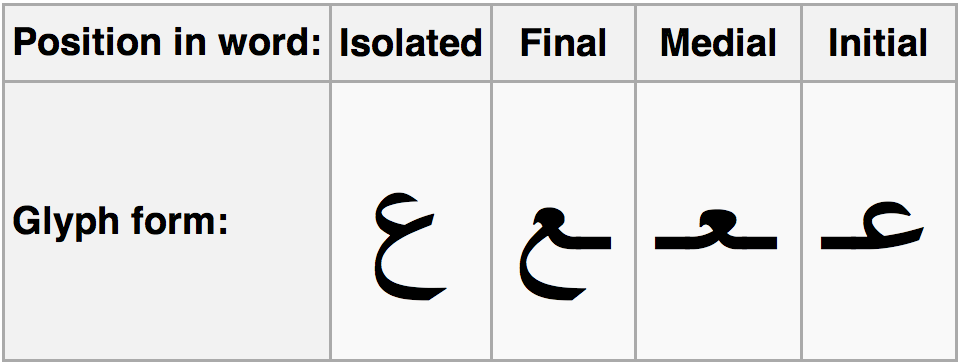
\includegraphics[width=1\textwidth]{img/arabicContextual.png}
                \end{figure}
            \end{columns}
            
            \vspace*{1em}

            \item Les voyelles peuvent être omises
            \item[] ...
        \end{itemize}
        \item Beaucoup d'autres langues (et de problèmes spécifiques!).
    \end{itemize}
\end{frame}
%-E--------------------------------------------------------------------------E-%

%##############################################################################%
\section{La problématique de la RI cross-lingue}
%##############################################################################%


%-B--------------------------------------------------------------------------B-%
\begin{frame}
    \frametitle{Introduction}
    \begin{itemize} \itemsep10pt
        \item La principale difficulté en RI cross-lingue et multilingue réside 
              dans la représentation des documents et des requêtes.
        \item Comment comparer des représentations construites à partir 
              d'informations disponibles dans différentes langues~?

        \begin{itemize} 
          \item[fr] Un \textcolor<2>{red}{Boeing 777} d'Asiana 
                    s'\textcolor<2>{JungleGreen}{écrase} à l'atterrissage à 
                    \textcolor<2>{blue}{San Francisco}.
          \item[en] \textcolor<2>{red}{Boeing 777} from Seoul 
                    \textcolor<2>{JungleGreen}{crashes} on landing at 
                    \textcolor<2>{blue}{San Francisco} airport.
          \item[jp] \begin{CJK*}{UTF8}{min}
                    \textcolor<2>{blue}{サンフランシスコ}国際空港で6日、
                    \textcolor<2>{red}{ボーイング777}型機が
                    \textcolor<2>{JungleGreen}{着陸に失敗し}、炎上した。
                    \end{CJK*}
        \end{itemize}
        \item[$\to$] Comment réussir à trouver les informations ci-dessus avec 
                     la requête ``\textcolor<2>{JungleGreen}{crash} d'un 
                     \textcolor<2>{red}{Boeing 777} à 
                     \textcolor<2>{blue}{San Francisco}''~?
    \end{itemize}
\end{frame}
%-E--------------------------------------------------------------------------E-%


%-B--------------------------------------------------------------------------B-%
\begin{frame}
    \frametitle{\textit{Mapping} entre les représentations}
    \begin{figure}
    \centering
    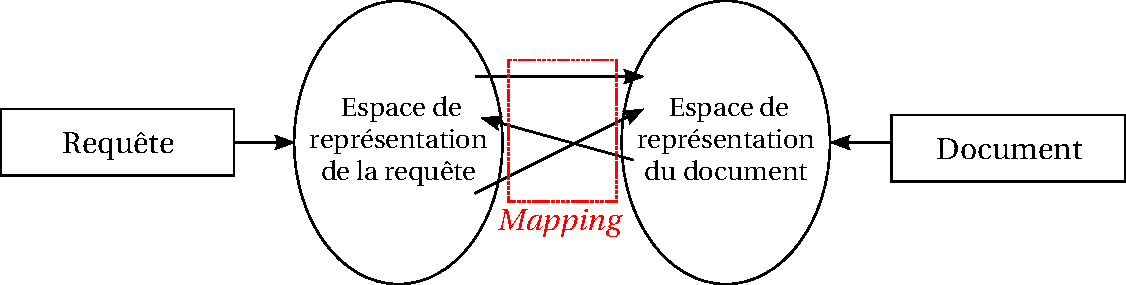
\includegraphics[width=1\textwidth]{img/mapping.pdf}
    \caption{\textit{Mapping} entre les représentations 
            (Figure 1.2 de~\cite{DBLP:series/synthesis/2010Nie}).}
    \end{figure}
    \vspace*{-1em}
    %
    \begin{enumerate} 
        \item \textit{Mapping} de la représentation du document dans celle de la
              requête~: approche par traduction de documents~\cite{oard1997}.
        \item \textit{Mapping} de la représentation de la requête dans celle du 
              document~: approche par traduction de requêtes.
        \item \textit{Mapping} des représentations de la requête et du document
              dans un troisième espace 
              (i.e.~langue pivot)~\cite{ruiz1999,Kishida:2005}.
    \end{enumerate}
\end{frame}
%-E--------------------------------------------------------------------------E-%


%-B--------------------------------------------------------------------------B-%
\begin{frame}
    \frametitle{Le processus de RI cross-lingue}
    \begin{figure}
    \centering
    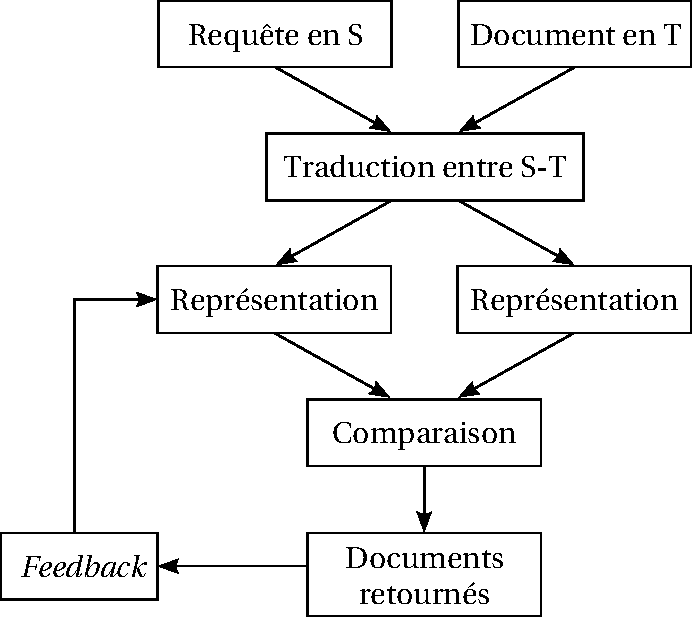
\includegraphics[width=0.65\textwidth]{img/typicalCLIR.pdf}
    \caption{Processus de RI cross-lingue (Figure 1.3 
             de~\cite{DBLP:series/synthesis/2010Nie}).}
    \end{figure}
\end{frame}
%-E--------------------------------------------------------------------------E-%


%-B--------------------------------------------------------------------------B-%
\begin{frame}[allowframebreaks]
    \frametitle{Traduction du document ou de la requête~?}
    \begin{itemize} \itemsep10pt
        \item Les méthodes par traduction de la requête sont plus flexibles.
        \begin{itemize}
            \item L'utilisateur peut choisir les langues des documents à
                  chercher.
            \item Dans le cas ou il est capable de comprendre la requête 
                  traduite, il peut la corriger ou l'étendre.
        \end{itemize}
        \item \textbf{Cependant}, la traduction automatique de la requête peut 
              être ambiguë de part la taille très limitée du contexte.
        \begin{itemize}
            \item Erreurs de segmentation pre-traduction \\
                  \begin{CJK}{UTF8}{min}
                  任天堂 (nintendo) (jp) $\to$  任 (responsabilité) 天 (ciel) 
                  堂 (salle)
                  \end{CJK}
            \item Erreurs de (sur-)traduction \\
                  \textit{perfume japanese band} (en) $\to$ parfum groupe 
                  japonais (fr)        
        \end{itemize}

        \framebreak

        \item La traduction du document est plus robuste mais les travaux 
              précédents ne montrent pas de différence~\cite{McCarley:1999}.
        \begin{itemize}
            \item Les systèmes de traduction automatique n'utilisent qu'une 
                  partie du contexte riche du document (traduction phrase à 
                  phrase).
        \end{itemize}
        \item \textbf{De plus}, les documents doivent être au préalable traduits
              dans toutes les langues possibles.
        \begin{itemize}
            \item Irréaliste avec les capacités de calcul et de stockage 
                  actuelles.
        \end{itemize}
        \item[$\to$] La majorité des approches en RI cross-lingue utilisent donc
                     la traduction de requête.
    \end{itemize}
\end{frame}
%-E--------------------------------------------------------------------------E-%


%-B--------------------------------------------------------------------------B-%
\begin{frame}
    \frametitle{Utilisation d'une langue pivot}
    \begin{itemize} \itemsep10pt
        \item La traduction directe entre deux langues peut ne pas être possible
              dans le cas où il n'existe pas de ressources suffisantes.
        \item \textbf{Mais}, il y a peut-être des ressources disponibles entre 
              ces langues et une troisième langue (e.g.~l'Anglais).
        \item Deux approches sont possibles~:
        \begin{enumerate}
            \item Traduction de la requête et du document dans la langue pivot.
            \item Traduction de la requête ou du document dans la langue pivot 
                  puis dans la langue cible.
        \end{enumerate}
    \end{itemize}
\end{frame}
%-E--------------------------------------------------------------------------E-%


%##############################################################################%
\section{La traduction en RI cross-lingue}
%##############################################################################%


%-B--------------------------------------------------------------------------B-%
\begin{frame}[allowframebreaks]
    \frametitle{La traduction en RI cross-lingue}
    \begin{itemize} \itemsep10pt
        \item En plus des difficultés liées à la RI monolingue, la traduction 
              automatique (TA) est la difficulté principale de la RI 
              cross-lingue et multilingue.
        \item La TA peut être nécessaire dans deux étapes~:
        \begin{enumerate}
            \item Sachant une requête en langue A (source), si l'utilisateur 
                  recherche des documents en langue B (cible), les termes en 
                  langue A doivent être traduits en langue B.
            \item Une fois que l'ensemble des documents pertinents en langue B 
                  est retrouvé, l'utilisateur peut vouloir les traduire en 
                  langue A de façon à pouvoir les comprendre.
        \end{enumerate}

        \framebreak

        \item Les deux étapes de traduction ci-dessus sont très différentes.
        \begin{itemize}
            \item La seconde est une tâche classique de TA de document.
            \item \textbf{Cependant}, la TA n'est pas nécessairement un outil 
                  approprié pour la première étape.
        \end{itemize}
        \item \textbf{Une syntaxe moins stricte est nécessaire}
        \begin{itemize}
            \item La tâche de traduction d'une requête en RI cross-lingue 
                  n'est pas de la rendre lisible par un humain mais de permettre
                  au système de faire un \textit{matching}.
            \item[$\to$] La syntaxe/grammaire n'est donc pas très importante.
        \end{itemize}
        \item \textbf{Un niveau d'ambiguïté plus important}
        \begin{itemize}
            \item Les requêtes sont généralement très courtes (2-3 mots).
        \end{itemize}

        \framebreak

        \item \textbf{Un effet d'expansion de requêtes}
        \begin{itemize}
            \item Le but de la traduction de requête est de produire une 
                  représentation de cette dernière dans une autre langue.
            \item De manière à pouvoir \textit{matcher} les termes de la requête
                  avec ceux du document, il est préférable d'inclure toutes les
                  alternatives de traduction.
        \end{itemize}
        \item \textbf{La pondération des termes}
        \begin{itemize}
            \item Le poids assigné à chacun des termes de la requête reflète 
                  l'importance de ce terme lors du \textit{matching}.
            \item En RI cross-lingue, le poids d'un terme doit reflèter son 
                  importance mais également la qualité de la traduction.
        \end{itemize}

        \framebreak

        \item Dans la littérature, en plus de la TA, les deux approches 
              suivantes ont été largement testées et évaluées~:
        \begin{enumerate}
            \item Traduction basée sur dictionnaire~: les traductions possibles 
                  des termes sont issues d'un dictionnaire 
                  bilingue~\cite{Pirkola:2001}.
            \item Traduction basée sur un corpus parallèle~: utilise les 
                  relations de traduction entre deux langues des 
                  termes~\cite{Chen00parallelweb}.
        \end{enumerate}
        \item Il n'y a pas de séparation stricte entre les approches, 
              e.g.~certaines approches de TA utilisent des dictionnaires.
        \item[$\to$] En séparant les approches utilisant un système de TA, nous
                     mettons en avant le fait que les systèmes de TA sont dans la
                     plupart des cas utilisés comme une \textit{black box}.
    \end{itemize}
\end{frame}
%-E--------------------------------------------------------------------------E-%

%##############################################################################%
\section{L'utilité de la RI cross-lingue}
%##############################################################################%


%-B--------------------------------------------------------------------------B-%
\begin{frame}
    \frametitle{L'utilité de la RI cross-lingue et multilingue}
    \begin{itemize} \itemsep10pt
        \item Bien que le besoin de méthodes de RI monolingue ne soit plus à 
              démontrer, celui de méthodes cross-lingue et multilingue 
              peut apparaître moins évident.
        \item L'objectif en RI est d'identifier les informations pertinentes.
        \begin{itemize}
            \item La forme de la description de l'information n'a que peu
                  d'importance~: un texte, une image, un tableau, etc.
            \item Les informations ne sont utiles que si elles sont 
                  compréhensibles.
        \end{itemize}
        \item L'obstacle de la compréhension de documents dans une langue 
              différente est la raison pour laquelle les moteurs de recherche 
              actuels sont monolingues.
        \item[$\to$] \textbf{Cependant}, cet obstacle est en train de tomber 
                     avec les progrès faits dans les outils de TA.
    \end{itemize}
\end{frame}
%-E--------------------------------------------------------------------------E-%

%-B--------------------------------------------------------------------------B-%
\begin{frame}[allowframebreaks]
    \frametitle{Rechercher dans une autre langue}
    \begin{itemize} \itemsep10pt
        \item Indépendamment de la disponibilité des outils de TA, il y a 
              de nombreuses raisons de rechercher des documents sans égard pour 
              la langue.
        \item L'information recherchée peut être sous une forme directement 
              compréhensible (e.g.~image, tableau).
        \begin{itemize}
              \item[$\to$] Les méthodes de recherche d'images sont en grande 
              partie basées sur leurs descriptions textuelles.
        \end{itemize}
        \item L'information recherchée peut ne pas exister dans la langue de 
              l'utilisateur.
        \begin{itemize}
              \item[e.g.] Un anglophone intéressé par des informations sur un 
                    festival de danse traditionnelle bretonne.
        \end{itemize}
        
        \framebreak
        
        \item Les documents peuvent mélanger plusieurs langues.
        \begin{itemize}
          \item[e.g.] \begin{CJK}{UTF8}{min}
                      Internetの進化 (jp) ou インヌーネットの進化 (jp)
                      \end{CJK} \\
                      internet no shinka (évolution d'Internet)
        \end{itemize}
        \item Un utilisateur peut vouloir retrouver \textbf{toute} l'information
              pertinente, quelque soit la langue utilisée.
        \begin{itemize}
        \item[$\to$] Il s'agit de \textit{Recall-oriented retrieval}.
        \item[e.g.] Recherche de brevet (\textit{patent retrieval}), création 
                    d'état de l'art.
        \end{itemize}
        \item Un nombre important et croissant d'utilisateurs sont capables de 
              comprendre plus d'une langue.
        \begin{itemize}
        \item[$\to$] Un système de RI cross-lingue ou mutlilingue peut faciliter
                    l'accès aux informations (pas besoin de traduire la requête).
        \end{itemize}
    \end{itemize}
\end{frame}
%-E--------------------------------------------------------------------------E-%

%##############################################################################%
\section{Historique}
%##############################################################################%


%-B--------------------------------------------------------------------------B-%
\begin{frame}[shrink=5]
    \frametitle{Historique de la RI cross-lingue}
    \begin{itemize} \itemsep10pt
        \item Les premiers travaux sur la RI cross-lingue remontent aux 
              \textbf{années 60}~\cite{Salton:1969:APF:990403.990407}.
        \item Le nombre de travaux a sérieusement augmenté au milieu des 
              \textbf{années 90}, lorsque le Web a commençé à être populaire.
        \item \textbf{1997}, première campagne d'évaluation TREC (\textit{Text 
              REtrieval Conference}) en RI cross-lingue est organisée par le 
              NIST (\textit{National Institute of Standards and 
              Technology})~\cite{Voorhees:2000:OST:342528.342531}.
        \item \textbf{1999}, expérimentations sur les langues asiatiques 
              débutent avec l'atelier NTCIR organisé par le NII 
              (\textit{National Institute for Informatics}).
        \item \textbf{2000}, expérimentations sur les langues européennes 
              débutent avec CLEF (\textit{Cross-Language Experiment Forum}).
    \end{itemize}
\end{frame}
%-E--------------------------------------------------------------------------E-%


% %-B--------------------------------------------------------------------------B-%
% \begin{frame}
%     \frametitle{}
% \end{frame}
% %-E--------------------------------------------------------------------------E-%

\appendix


%##############################################################################%
\section*{Références}
%##############################################################################%


%-B--------------------------------------------------------------------------B-%
\begin{frame}[allowframebreaks]
    \fontsize{9pt}{10}\selectfont
    \frametitle{References}
    \bibliographystyle{alpha}
    \bibliography{bibliography}
\end{frame}
%-E--------------------------------------------------------------------------E-%


\end{document}